% Latex template: mahmoud.s.fahmy@students.kasralainy.edu.eg
% For more details: https://www.sharelatex.com/learn/Beamer

\documentclass[aspectratio=1610]{beamer}					% Document class

\setbeamertemplate{footline}[text line]{%
  \parbox{\linewidth}{\vspace*{-8pt}Semantic Segmentation with UNET \hfill\insertshortauthor\hfill\insertpagenumber}}
\setbeamertemplate{navigation symbols}{}

\usepackage[english]{babel}				% Set language
\usepackage[utf8x]{inputenc}			% Set encoding

\mode<presentation>						% Set options
{
  \usetheme{default}					% Set theme
  \usecolortheme{default} 				% Set colors
  \usefonttheme{default}  				% Set font theme
  \setbeamertemplate{caption}[numbered]	% Set caption to be numbered
}

% Uncomment this to have the outline at the beginning of each section highlighted.
%\AtBeginSection[]
%{
%  \begin{frame}{Outline}
%    \tableofcontents[currentsection]
%  \end{frame}
%}

\usepackage{graphicx}					% For including figures
\usepackage{booktabs}					% For table rules
\usepackage{hyperref}					% For cross-referencing
\usepackage[absolute,overlay]{textpos}
\usepackage{bm}

\title{Semantic Segmentation of Nuclei with U-NET}	% Presentation title
\author{Clayton W. Seitz}								% Presentation author
\date{\today}									% Today's date	

\begin{document}

% Title page
% This page includes the informations defined earlier including title, author/s, affiliation/s and the date
\begin{frame}
  \titlepage
\end{frame}

\begin{frame}{Segmentation problem}

\begin{itemize}
\item Need a lot of data due to sample, batch, and real biological variability. 
\item Automating segmentation
\item Simple thresholding/watershed do not work well over large FOV
\item Imprecise estimates of cell boundaries\\
\end{itemize}

\vspace{0.1in}

\textbf{But...} probably need a new model for every sample type. Worth the effort if we can achieve low validation loss with few training samples (few-shot learning)\\

\begin{center}
\begin{figure}
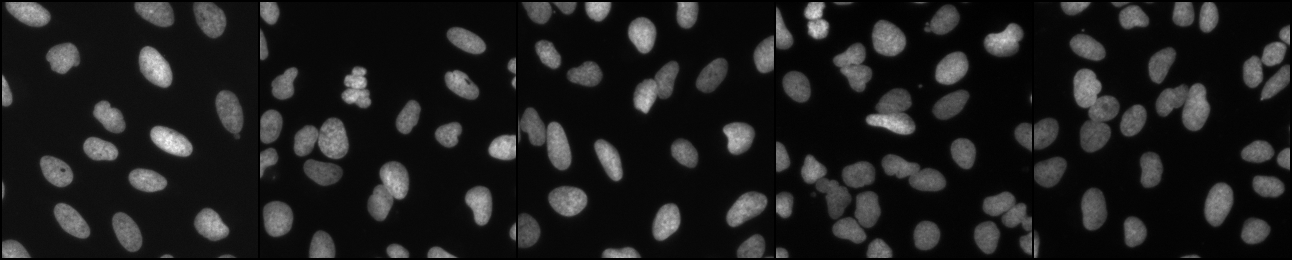
\includegraphics[width=0.85\textwidth]{input-train.png}
\caption{U2OS nuclei from BBBC039 dataset}
\end{figure}
\end{center}

\end{frame}

\begin{frame}{U-NET Architecture}

\begin{center}
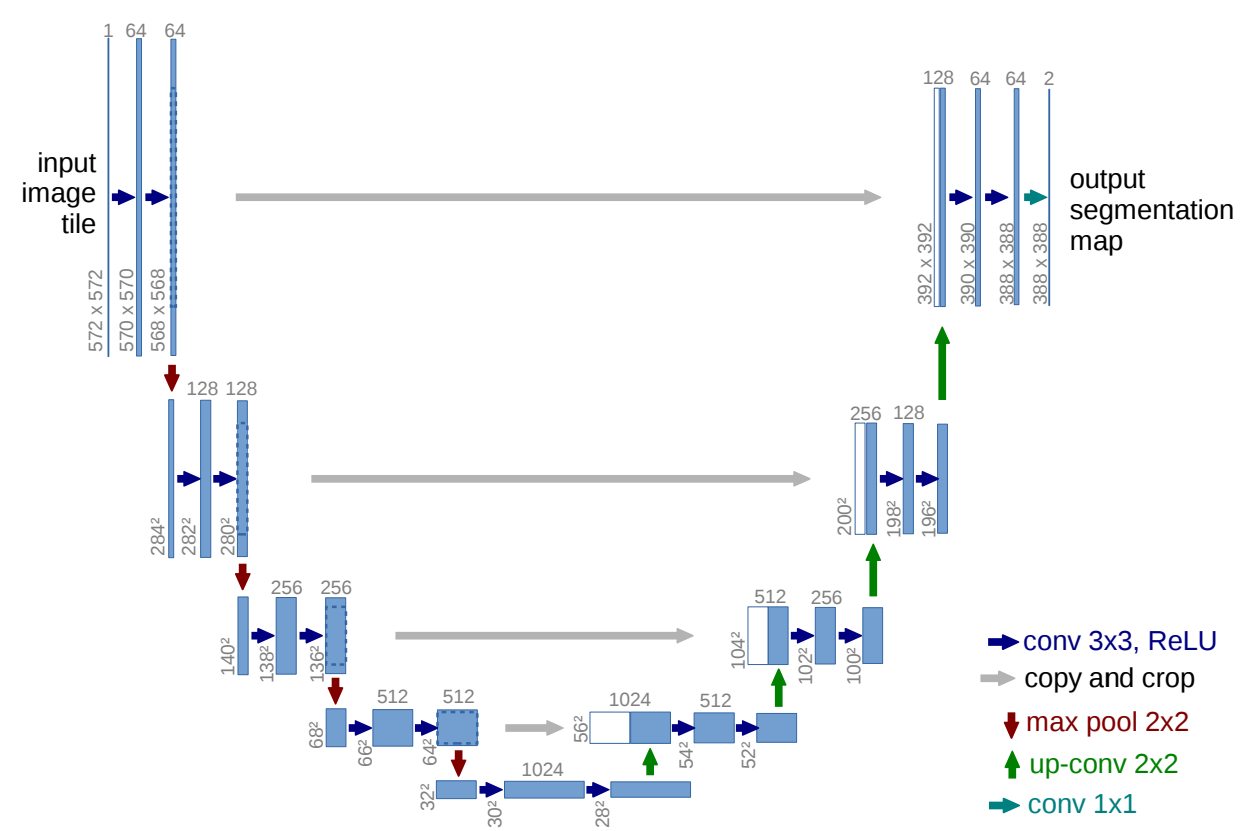
\includegraphics[width=0.75\textwidth]{unet.png}
\end{center}
\end{frame}

\begin{frame}{Training on BBBC039 U2OS Cells}
\vspace{0.1in}
BBBC039: 200 images, 160 train + 40 validation, 256\;x\;256 random crop

\begin{center}
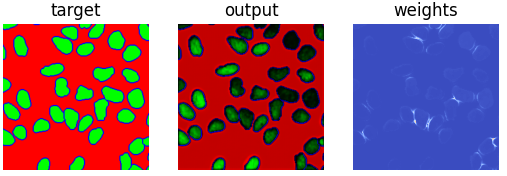
\includegraphics[width=0.8\textwidth]{weights.png}
\end{center}

We train a 3-channel semantic segmentation model with \textbf{weighted} cross-entropy loss:

\begin{equation*}
\mathcal{L} = \sum_{i,j} w_{ij}\log p_{ij}(\tilde{x}) = \sum_{i,j} w_{ij}\log \frac{\exp(-s_{ij}(\tilde{x}))}{\sum_{x\in\chi} \exp(-s_{ij}(\tilde{x}))}
\end{equation*}

$p_{ij}$ is the probability the model assigns a pixel to the true class $\tilde{x} \in \{\textrm{a}, \textrm{b}, \textrm{c}\}$

\end{frame}

\begin{frame}{Training on BBBC039 U2OS Cells}

\begin{center}
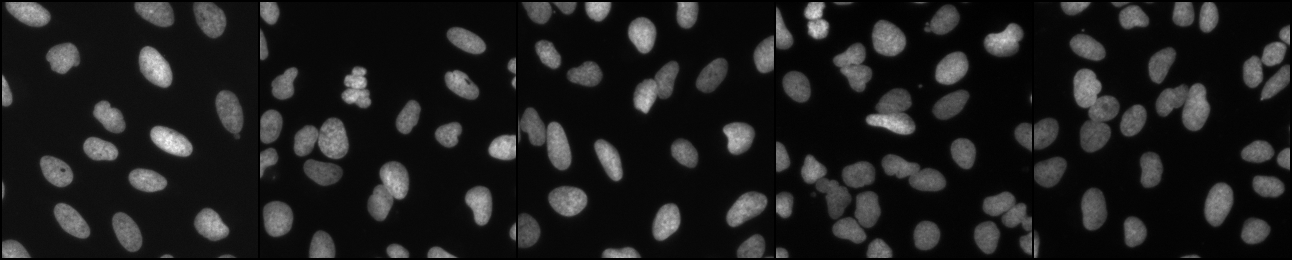
\includegraphics[width=0.85\textwidth]{input-train.png}
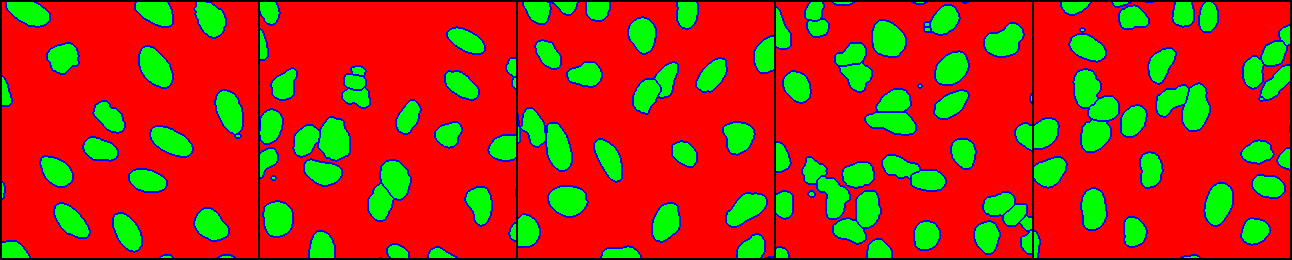
\includegraphics[width=0.85\textwidth]{target-train.png}
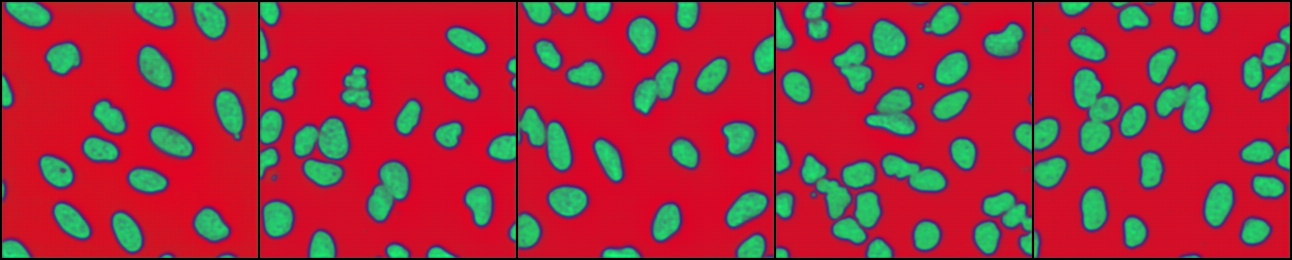
\includegraphics[width=0.85\textwidth]{output-train.png}
\end{center}

\end{frame}

\begin{frame}{Training on BBBC039 U2OS Cells}
Learning rate $\eta=0.01$, Batch-size $B=5$ (32 train iterations, 8 validation)
\begin{center}
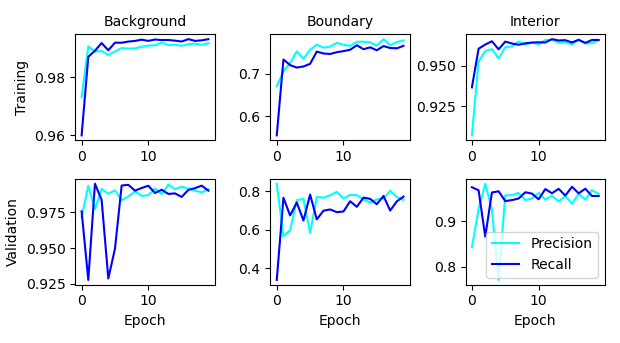
\includegraphics[width=0.85\textwidth]{metrics.png}
\end{center}

\end{frame}
\end{document}
